\documentclass[9pt,conference]{IEEEtran}

\usepackage[colorlinks,allcolors=blue]{hyperref}
\usepackage{listings}
\usepackage{graphicx}
\usepackage{amsfonts}
\usepackage{verbatim}
\graphicspath{{./images/}}

\begin{document}

    \title{Quality assurance of digital twins -- An experience report in the automotive industry}
    \author{
        \IEEEauthorblockN{
            Georg Hackenberg
        }
        \IEEEauthorblockA{
            School of Engineering\\
            University of Applied Sciences Upper Austria\\
            4600 Wels, Upper Austria, Austria\\
            \href{mailto:georg.hackenberg@fh-wels.at}{georg.hackenberg@fh-wels.at}
        }
        \and
        \IEEEauthorblockN{
            Alican Tüzün
        }
        \IEEEauthorblockA{
            School of Engineering\\
            University of Applied Sciences Upper Austria\\
            4600 Wels, Upper Austria, Austria\\
            \href{mailto:alican.tuezuen@fh-wels.at}{alican.tuezuen@fh-wels.at}
        }
    }
    \maketitle

    \begin{abstract}
        Digital twins are becoming more and more important for the efficient and effective development and operation of cyber-physical systems.
        However, digital twins are only useful if they reflect the real-world system accurately enough, i.e.\ their quality is high enough.
        This claim entails the question, of what the term quality in the context of digital twins means and how it can be measured.
        In this article, we present our experience with the quality assurance of a digital twin for an assembly line in the automotive industry.
        We explain our preliminary definition of digital twin quality, which we derive from classical quality models for general software systems.
        Furthermore, we describe quality issues, which we were able to detect in a digital twin of an assembly line in the automotive industry.
        Finally, we conclude how to leverage our experience in different contexts and how to generalize the underlying approaches.
    \end{abstract}

    \section{Introduction}\label{section:introduction}
    A popular but highly misunderstood notion with fuzzy boundaries is the `digital twin.' 
    The misunderstanding began with the Apollo 13 mission, which many authors claim, had a first digital twin. The twin of Apollo 13 was merely a tangible replication of the spacecraft that has been utilized in physical simulations. Even though the `digital' aspect was expected to be present, 
    it wasn't~\cite{GrievesApollo13}. The historic D-day map (also known as the Big Board) in Southwick House England, which was used simultaneously before and during operation, can be argued to be similar. 
    The board was a twin of the operation, and it included models of battalions and ships that reflected the actual locations of the corresponding formations. 
    Furthermore, synchronization was implemented with radio communication to give directives from the real system to control the operation flow and also to update the twin's state~\cite{AMRC}.

    To begin analyzing `the digital twin' and its quality, authors needed to come up with a concrete description that involved a great level of abstraction. 
    The definition of a digital twin given by the digital twin consortium, according to the authors, is the best one currently available: `A digital twin is a virtual representation of real-world entities and processes, synchronized at 
    a specified frequency and fidelity.'~\cite{digitaltwinconsortium2022}.

    Why do we assume this definition to be the best? Because it provides the highest abstraction level among the definitions of digital twins that we discovered during our literature analysis. The following is a poor example of abstraction taken from the initial definition of a digital twin from NASA's roadmap from 2010: `A digital twin is an integrated multi-physics, multi-scale, probabilistic simulation of a 
    vehicle or system that uses the best available physical models, sensor updates, fleet history, etc., to mirror the life of its flying twin~\cite{NASA}.'
    The digital twins that we encounter nowadays don't typically fall under NASA's definition. We want to stress that NASA's definition of a  digital twin is accurate since digital twins are systems that are `context' centered. 
    Therefore, this definition is appropriate in the context of NASA's use case and is thus accurate, but the abstraction level is not sufficiently high to allow for a thorough understanding of digital twins.

    In addition, we emphasize the significance of Grieves' 2006 description of digital twins in the PLM book,
    which traces the origins of the concept. Although it featured the same components as a digital twin at the time, it was known as an Information Mirroring Model (IM)~\cite{GrievesPLMBook}. 
    They decided to use NASA's Digital Twin rather than IM after co-authoring the article with Vickers.

    \begin{figure}
        \centering
        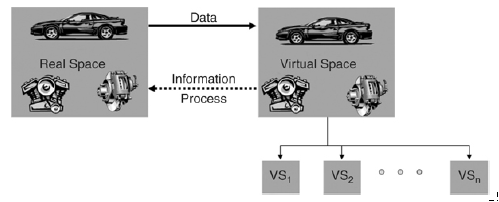
\includegraphics[width =0.45\textwidth]{GrievesInformationMirroringModel.png}
        \caption{Grieves Information Mirroring Model}\label{fig:GrievesInformationMirroringModel}
        \cite{GrievesPLMBook}
    \end{figure}

    \subsection*{Real System}

    The term `real system' in the context of digital twins refers to a system that is a tangible thing that has the characteristics of a system. Depending on the system's context, we can use black-box, gray-box, or white-box methodologies to study the system. 
    The use of various artifacts by Grieves in a system he referred to as `real space' can be seen in Figure~\ref{fig:GrievesInformationMirroringModel}.

    \subsection*{Virtual System}
    Virtual refers to an existence that exists in a computer system, as opposed to a physical system. Therefore, virtual systems are abstract systems, which are nothing but an abstraction of the real system.
    The term `abstract systems' refers to systems that have had their set of variables and functions `abstracted' so that they may be computed by a solver, which in this case, a solver could be either the human brain or a computer.
    Additionally, just because a system is an abstract system doesn't mean it lacks a physical body; rather, it is abstracted. 
    Virtual systems can't exist on their own since, like abstract systems, they require a medium to exist. Computer systems, a higher system of virtual systems, are an ideal medium for virtual systems.
    
    \subsection*{Connection Between the Real and Virtual System}
    If we step back and observe the consortium's definition in Section~\ref{section:introduction}, which we assumed, was the best definition we could find, 
    it mentions synchronization, fidelity and some specified frequency. As can be guessed these terms are attributes of the real-virtual connection.
    Synchronization is used here instead of twinning, mirroring and connecting. 
    Real-time is a time value, which is most of the time a constant value and defines the update frequency of the state of the virtual system of interest relative to the system of interest.
    Fidelity is the degree of precision and accuracy of our digital twin, relative to the system of interest.
    These words are highly dependent on the context of the digital twin.
    \subsection{Research objective}
    Find an approach to assess the quality of Digital twins~\cite{Jones2020}

    \subsection{Research question}\label{section: Research Questions}
    What is the quality of digital twins?
    What is the state art of digital twin quality?

    \subsection{Research methodology}
    TODO

    \section{State of the art on quality}
    In the Oxford English Dictionary, the word `quality' is described as a noun as well as an adjective. The Adjective form indicates, a high standard or excellence. 
    For example, the phrase `quality products' implies that quality adds a high standard state to the product. 
    There are several meanings for the noun, but the one that interests us in this situation is `the standard of something as measured against other things of a similar kind. \cite{OxfordDictionary}'
    This definition shows the relativity of quality.

    According to ISO 9000:2015, quality is the degree to which a set of inherent characteristics of an object fulfills requirements~\cite{ISO9000}. Several words need to be expanded, to understand this definition. 
    
    First, the standard also explains characteristics as distinguishing features such as physical, sensory, behavioral, temporal, ergonomic and functional. 
    Instead of an object, a system can be used for more generalization.
    As for the requirements, the standard also explains as a requirement is a need or expectation that is stated, generally implied or obligatory.~\cite{ISO9000}

    Thus, when these definitions are combined, we obtain the following: `Quality is a degree to which a set of inherent distinguishing features of a system fulfills a need or expectation that is stated, generally implied or obligatory'. 
    It should be highlighted that there are various quality definitions by so-called `Quality Gurus', but the authors decided to expand the standard definition of ISO 9000.

    \subsection*{Product quality and Management}
    A product is a tangible or intangible system that satisfies the needs or wants of a customer. It could be a physical system like a car, or an abstract system, like a digital twin. 
    Regarding product quality, there are two different aspects~\cite{GrievesPLMBook}.
    First, quality is an attribute of a product, which meets product specifications. Specifications are mostly defined by the supra-systems subsystems, such as by the stakeholders within the supra-system,  If the stakeholders' expectations, or needs, are met, we can consider high quality.
    The ability to execute to a specific usage standard is the second facet of product quality. Since this standardization is usually not controllable, unlike the first, the system's quality will be determined by how the implied or obligatory standards are fulfilled.

    Quality management is a management type, which has an interest in Quality, and quality assurance is one of the parts of quality management, 
    which focuses on providing fidelity that quality requirements will be fulfilled. This means that quality assurance is a subsystem of quality management.

    Quality management systems(QMS) are being used to plan and execute the organization's quality policies and goals. 
    Examples of such systems can be a standard like ISO 9001 which can provide a framework for an organization, or a data-driven methodology 
    such as Six Sigma to reduce defects and improve efficiency. These concepts are not new, for example, ISO 9001 standard has been established in 1987, 
    and is still being regularly updated~\cite{ISO9001DebunkingtheMyth}.

    \subsection*{Software quality}
    Software is a  virtual system, which has a set of instructions, data or programs used to perform a specific task. 
    All virtual systems, which we described above, need a medium to live on, hence these systems can be found in a computer or other electronic device.  
    Software quality according to IEEE 730-2014, is: 
    `The degree to which a software product meets established requirements; however, 
    quality depends upon the degree to which those established requirements accurately represent stakeholder needs, wants, and expectations'~\cite{IEE730-2014}. 
    As can be seen, it's a generic explanation of a quality, which doesn't differ much from the explanation we gave above. 

    Software quality management techniques come from already used manufacturing techniques in the industries.
    For example, the quality assurance that we mentioned above, also has been used as a software quality management activity with some differences. 
    In manufacturing, products will never exactly meet a specification, due to errors in the machining so there should be some tolerance for the manufacturing. 
    But in the software systems, or more precisely in the virtual systems, it's most of the time, not the case. 
    Also its nearly impossible to conclude that, the software product fully meets its specifications\cite{SoftwareEngineering}.

    According to ISO/IEC:25010:2011, there are eight software quality attributes. Functional Suitability, 
    Performance efficiency, compatibility, usability, reliability, security, maintainability and portability.\cite{ISO/IEC:25010}
    Of course, not all aspects can be inspected and the person, who is responsible for the quality of the product, should choose the critical aspects of the software product and further the process according to that decision.

    \subsection*{Simulation Quality}
    Simulation models are not merely virtual systems; they are also abstracted systems, which are nothing more than imitations or, to be more precise, abstractions of real systems. 
    We are simulating something every day when we are trying to predict the future outcome or abstractly thinking about the past state of some occurred event. 
    An important element to remember is that we mentally model the event before executing the simulation. However, most of the simulation processes we see today, 
    are computer-based, with software programs. These programs include ANSYS\cite{Ansys}, ABAQUS\cite{Abaqus}, and AnyLogic\cite{AnyLogic}, as examples. Consequently, the idea of simulation software programs emerges.

    Validation and verification can be used to evaluate the quality characteristics of the simulation model \cite{StewartSimulation} \cite{VerificationValidationSergent} \cite{OsmanBalci}. 
    Validation is the process of evaluating the simulation quality of the model in comparison to the real system from the perspective of the model's intended applications. 
    On the other hand, verification is a procedure to evaluate a simulation model's implementation and its associated data concerning the conceptual description and specifications of the model developer. 

    \subsection*{Digital twin quality}
    To analyze the state of the digital twin quality, a literature analysis was executed. 
    The analysis especially focused on how the digital twin quality is mentioned and assessed within the academic dissertations.

    \subsubsection*{Literature Search Methodology}
    Google Scholar (GS), Scopus (SCP) and Research Rabbit (RR) tools are used to fulfill our requirements for the literature review. Since there is a great number of digital twin publications in academics,
    narrowing the research is necessary, so the following algorithm with two levels of filtering will be applied.

    Initial filtering has been done with the following criteria
    \begin{itemize}
        \item  Dissertations should be written in English and published in a journal/conference.
        \item  Search term should be exactly searched
    \end{itemize}
    Filtering query calls for the GS and SCP are the following
    \begin{itemize}
        \item Google Scholar = `search term'
        \item Scopus = ALL (`digital twin quality') AND (LIMIT-TO (LANGUAGE, `English'))
    \end{itemize}
    After the initial filtration, the second filtering which is a manual investigation should occur with the following filtering criteria:
    \begin{itemize}
        \item  Remove Duplications
        \item  Remove the dissertations which are not English
        \item  Proper literature review should be present in the selected dissertation
        \item  Abstract and conclusion should be relevant to the search term
    \end{itemize}

    If an interesting dissertation(s) would be found during the reading, it will be checked again with the initial filter.

    \subsection*{Literature Result}
    The search term `digital twin quality' initially yielded 41 results on Google Scholar and three on Scopus. 
    After the second filtering stage, six duplicate dissertations were removed, along with ten dissertations that were not in English. As a result, only nine dissertations passed all the criteria and were inspected, while the remainder were rejected.
    
    The search term `digital twin verification' initially yielded, resulting in nineteen hits on Google Scholar and zero on Scopus. After the second filtering stage, one duplicate dissertation was removed, along with two dissertations that were not in English.
    As a result, all dissertations were rejected. 

    The search term `digital twin validation' was filtered initially, resulting in fifty-nine hits on Google Scholar and zero on Scopus. After the second filtering stage, four duplicate dissertations were removed, along with 4 dissertations that were not in English.
    As a result, eight dissertations passed all the criteria and were inspected while the remainder were rejected.

    \subsection*{Findings}

    The findings are the following;
    \begin{itemize}
        \item Shcherba et al. center their attention on the model quality, which is an observation for a digital twin subsystem. Despite being a crucial component of the digital twin, models alone cannot be used to assess the quality of the digital twin~\cite{Shcherba}.
        \item A consistency evaluation approach for digital twin models was developed by He Zhang et al. and can be used to assess the quality of the models. Additionally, 
        the authors discuss crucial ideas like consistency between real and virtual systems and ultra-fidelity models. The improvement of the service component is the primary emphasis of this article. Tao's five-dimensional digital twin concept includes this component~\cite{ZHANGEVALUATIONMETHOD}.
        \item He Zhang et al. introduces the updating method for digital twin models in yet another insightful article. Once more, the accuracy and coherence of the model concepts were addressed~\cite{ZHANGUPDATEMETHOD}.
        \item Selch et al. work is the only one that discusses the quality of the digital twin. The paper presents a machine-learning approach based on Bayesian networks to track the quality of the digital twin. The unique aspect of this study is that the author, rather than just analyzing the digital twin as a single system, determines the contributions of subsystems to forecast the overall quality of the digital twin. The digital couplings, which are linkages between the subsystems, are also mentioned by Selch et al. as a source of extra uncertainty. 
        Since only one digital twin has been used in practice, multiple subsystem digital twins have not been validated~\cite{QualityMonitoringofCoupledDigitalTwins}.
        \item The stability of the digital twin models was assessed using the Kolmogorov-Smirnov statistical test, which measures the degree of similarity between the probability distribution of the model's predictions and the distribution of the actual data~\cite{RadarDigitalTwin}.
        \item Edward Y. Hua et al. identify five open problems with digital twin model validation, including modeling realism, data uncertainty, system dynamics, use-case alignment, and reporting invalid modes. To address these challenges, the authors propose a digital-twin model validation framework. Additionally, the paper highlights three areas for future research, 
        including uncertainty and sensitivity analysis, model validation of system-of-systems, and combining expert knowledge and collected data~\cite{ValidationofDigitalTwins}.
        \item Shotaro Hamato et al. demonstrated real-time anomaly detection was successfully demonstrated using the Unscented Kalman Filter with the digital twin model, but determining the appropriate threshold for anomaly detection remains an issue~\cite{JapeneseKalmanFilterCorrectness}.
    \end{itemize}

    \section{Initial approach in the FELICE project}
    FELICE addresses a critical problem in robotics which is the effective integration of human and robot abilities in a collaborative setting. This challenge requires the development of sophisticated algorithms and techniques that facilitate seamless communication, 
    cooperation, and coordination between humans and robotic agents. By addressing this issue, FELICE tries to represent a 
    significant advancement in the field of robotics and has the potential to enhance the effectiveness and efficiency of a wide range of human-robot collaborative tasks with the consideration of safety~\cite{FELICE}.

    In the present study, we inspected several artifacts to evaluate the quality of the digital twin for the FELICE project, which is currently in the design phase. These artifacts included process videos showing the current assembly procedure, a scope definition, a requirements specification, a general and operational conceptual model, 
    and a discrete event simulation module. We assessed the quality of these artifacts based on four crucial quality attributes: correctness, completeness, fidelity, efficiency, and evolvability.

    \subsection{First criterion: Correctness}
    Correctness is a  derived word from the adjective correct, which means that something is error-free regarding a fact or truth~\cite{OxfordDictionary}. 
    In the context of the digital twins, our fact or truth is a real system hence, correctness is a grade of quality, that indicates an error between the real system and a digital twin system.
    Meanwhile, the quality of being correct is described by the term accuracy. Another important word is precision, 
    which refers to the ability to be precise and accurate\cite{OxfordDictionary}. 
    From a technical standpoint, we use precision in mathematics by the number of provided digits. 
    For instance, binary64 has 53 significant digits while binary32 has 24, displaying the precision of the structure~\cite{IEE754}.  
    
    \subsection{Second criterion: Completeness}
    According to the Oxford Dictionary, `complete'  can function as an adjective, attribute, or verb with an object\cite{OxfordDictionary}. When used as an adjective, it describes something 
    as having all the necessary or appropriate parts. To evaluate the completeness of a digital twin, 
    one must first analyze and synthesize the real system to identify subsystems and their relations with related systems in the supra-system. 
    After this initial analysis, completeness can be assessed by comparing the subsystems and relations of the real world with those of the digital twin.


    \subsection{Third criterion: Fidelity}
    The concept of fidelity has garnered significant attention in recent years and continues to be an important area of research in digital twins.
    In the context of digital twins, Fidelity refers to the degree of exactness with which the real system is copied and represented.
    Low-fidelity indicates a simplified representation, while high-fidelity refers to an accurate and detailed representation of the real system.
    This quality attribute plays a crucial role in evaluating the effectiveness of digital twins in accurately capturing the behavior and properties of real-world systems. 
    \subsubsection*{Fidelity vs Correctness}
    Correctness is a functional quality attribute, which assesses the behavior of the digital twin systems, by how accurately the results with the given precision match the behavior of the real system or more
    specifically outputs with the same given inputs. 
    This quality attribute focuses on the behavior of the system.
    On the other hand, fidelity is another quality attribute to consider. 
    It deals with the level of exactness and detail in the digital twin system's representation. 
    Fidelity concerns itself, with how the digital-twin system is exactly relative to the real system with a certain level of detail, which is more to do with the depiction or representation of the digital twin systems, rather than their behavior of them.

    \subsection{Fourth criterion: Efficiency}
    Efficiency refers to the quality of being efficient, and efficiency can be explained as achieving maximum productivity with minimum wasted effort or expense. 
    The concept of efficiency is tightly coupled with productivity, which refers to the quality of being productive. The word productive can be explained as producing or being able to produce large amounts of goods~\cite{OxfordDictionary}.
    For example, time efficiency indicates that,  with less amount of time as an input, more output with the minimum waste during the process is desired. Goods of the digital twin are nothing but information, 
    which Grieves first indicated with his Information Mirror Model~\cite{GrievesPLMBook}. So to assess the efficiency, one should inspect the sinks and sources of the digital twin system, to identify the waste, expense and productivity. 

    \subsection{Fifth criterion: Evolvability}
    A system's capability to enhance its suitability to its environment through alterations to both its internal and functional structure is referred to as evolvability. Another term used to describe the response to changes in the environment is adaptability. 
    However, this concept differs from evolvability in that it only affects a system's internal or functional structure temporarily. In contrast, evolvable systems undergo definite changes in their structures.  
    For instance, a digital twin, which is a virtual system, can be designed to be more flexible and scalable, allowing for easy updates and the addition of new features. 
    These updates and new features will result in definite changes to the structure of the system. On the other hand, a responsive web design is an adaptable system, capable of adjusting its size and layout depending on the user's hardware. 
    As we have seen in~\cite{ZHANGUPDATEMETHOD}, the update method shows that digital twins are evolvable systems,
    hence this attribute should be considered when the digital twin's quality is inspected. To assess the evolvability attribute, scalability analysis, reusability analysis, modifiability analysis, testability analysis, and maintainability analysis can be performed. 


    \begin{figure}[htbp]
        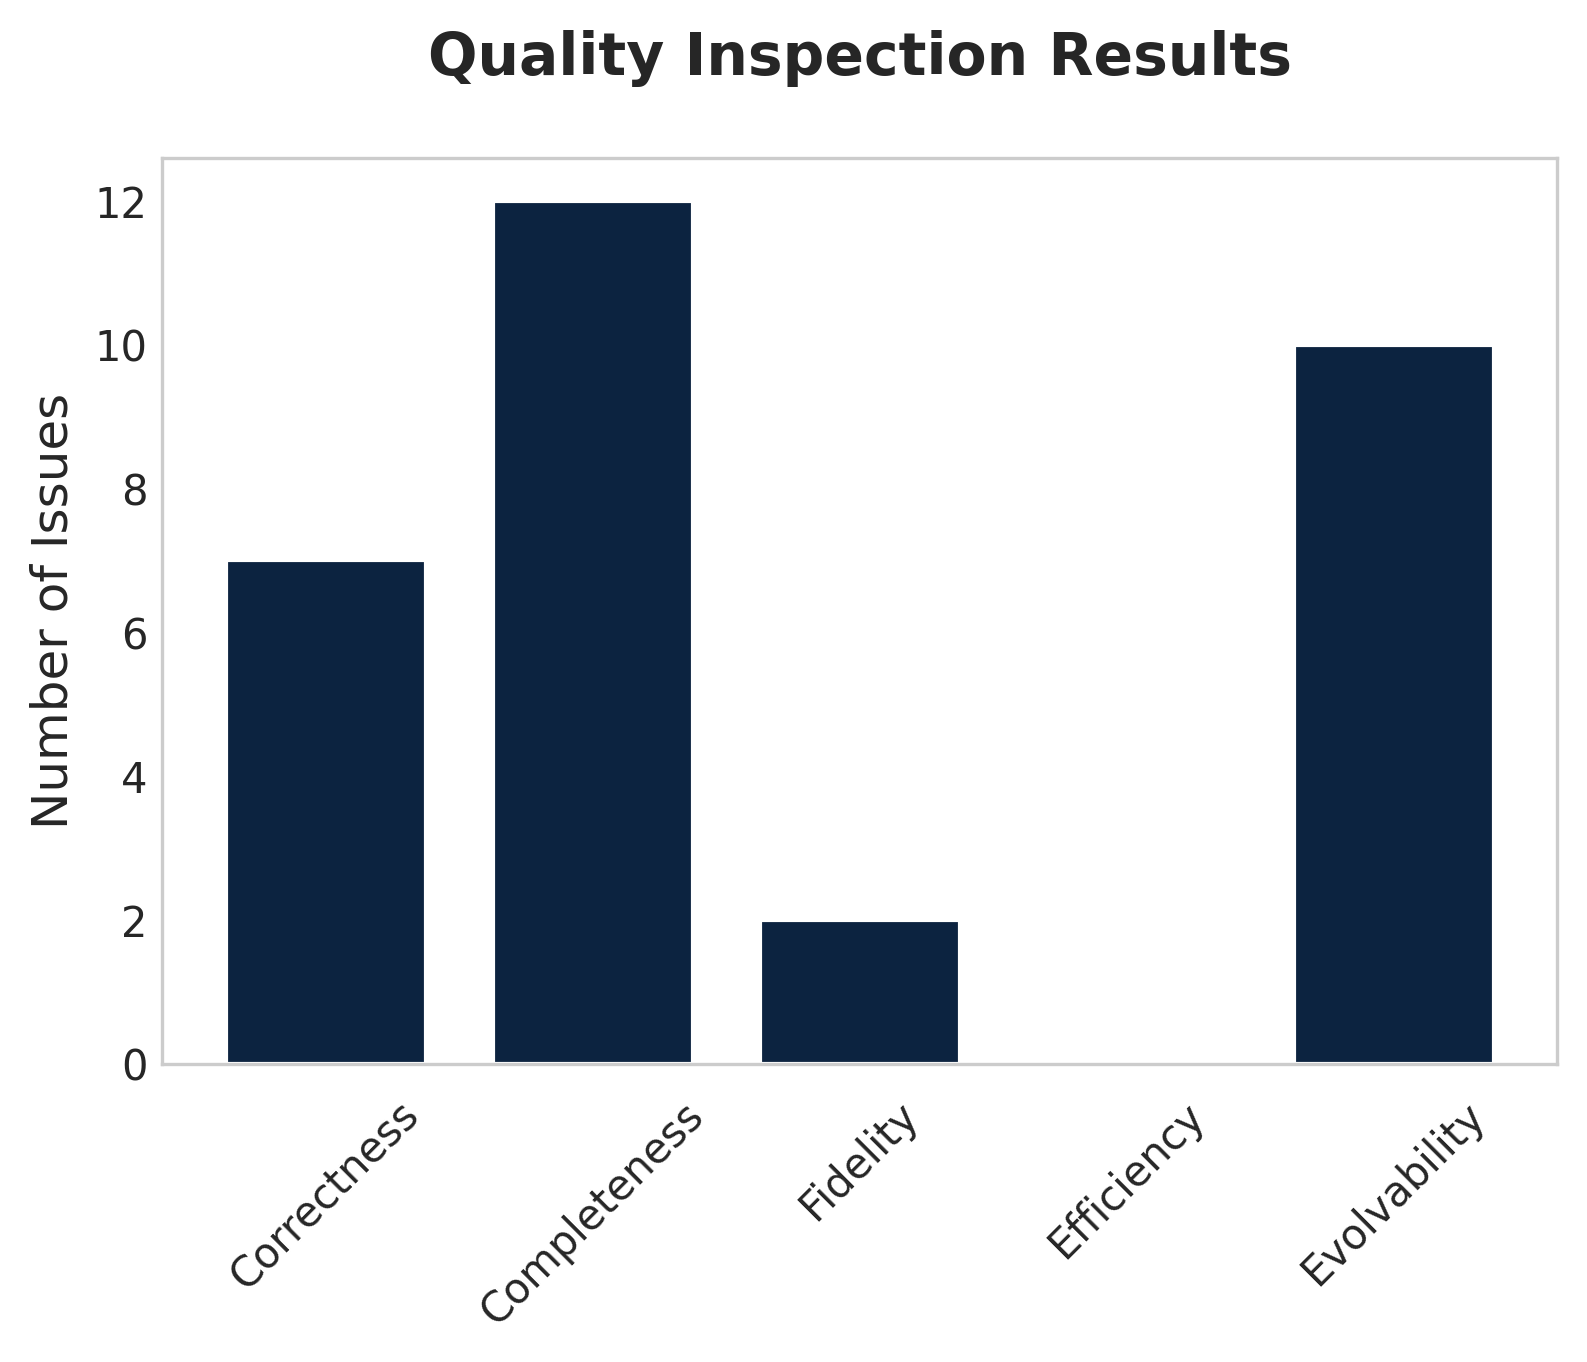
\includegraphics[width=\columnwidth]{quality_inspection_results.png}
        \caption{Overall Quality Inspection Results}
        \label{fig:QualityInspectonResults}

    \end{figure}\begin{figure}[htbp]
        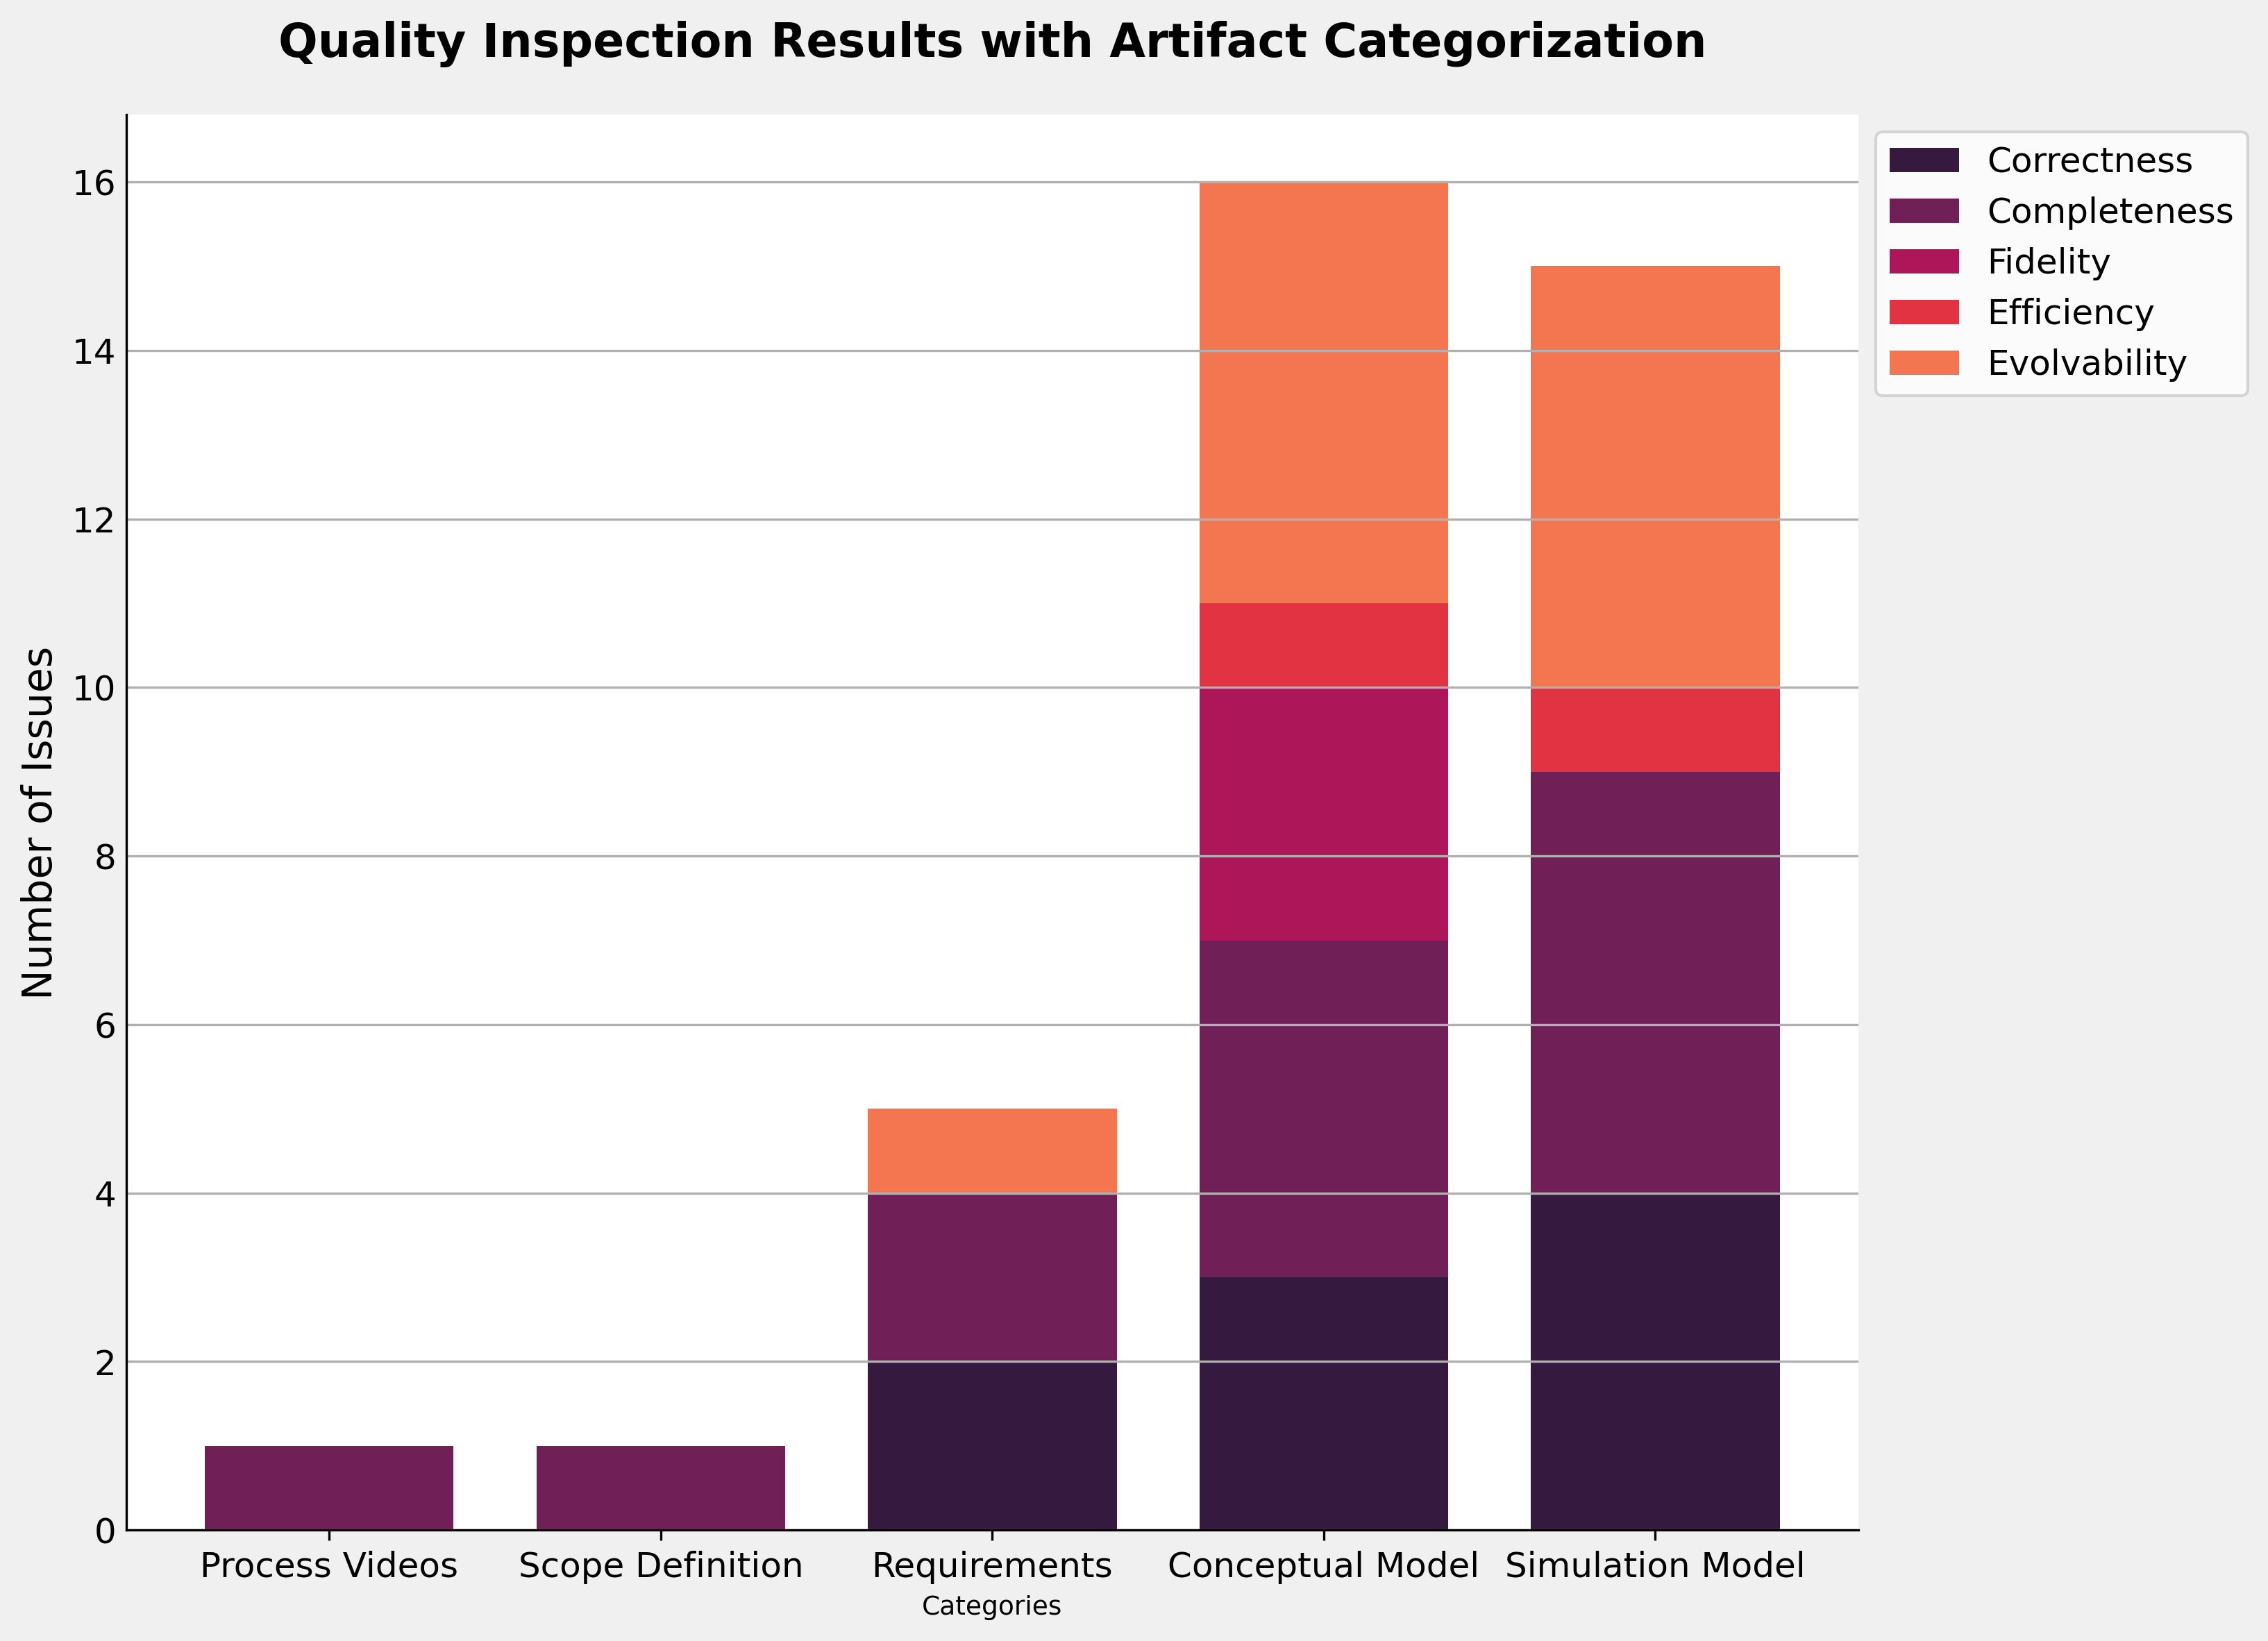
\includegraphics[width=\columnwidth]{quality_inspection_results_with_artifacts.png}
        \caption{ Quality Inspection Results Categorized with Artifacts}
        \label{fig:QualityInspectonResultsWithArtifacts}
    \end{figure}

    As can be seen in Figures ~\ref{fig:QualityInspectonResults} and ~\ref{fig:QualityInspectonResultsWithArtifacts}, based on our inspection of the given artifacts,
    we have identified a total of seven correctness issues, eleven completeness issues, and two fidelity issues. 
    It is important to note that we were unable to inspect for efficiency as the project is still in the design phase, 
    and we do not have enough data to make estimations for this attribute. Additionally, all of our inspections were conducted manually, 
    which is susceptible to human error and inspector bias.


    \subsection{Future approach in the FELICE project}
    \label{section:framework_1}
    To mitigate potential human bias and enhance the data-driven approach for quality assurance, ongoing research aims to address these issues. 
    Furthermore, the assessment of digital twin quality can be significantly improved by obtaining data from real systems, thereby enabling better visibility and a more robust evaluation. As such, the use of empirical data in combination with machine learning techniques can offer a more objective and reliable means of evaluating the correctness, completeness, fidelity, efficiency, and evolvability of digital twins. Additionally, given the manual nature of the current inspections, it is important to acknowledge the potential for inspector bias, which may impact the accuracy of the assessments. 
    By leveraging technology to automate certain aspects of the evaluation process, it is possible to reduce the potential for such biases and improve the overall quality of digital twin assessments.

 
    \section{Conclusion}~\label{section:conclusion}
    The success of the digital twin system depends on its quality, which requires careful evaluation based on several crucial quality attributes. The correctness of the system is measured by how accurately it behaves compared to the real system.
    Completeness assesses whether the digital twin's subsystems and relations match those of the real system. 
    Fidelity refers to the degree of exactness with which the real system is copied and represented.
    Efficiency measures the productivity of the system and the minimum waste during the process. 
    Evolvability is the system's ability to enhance its suitability to its environment through alterations to both its internal and functional structure. 
    Evaluating these quality attributes of the FELICE digital twin system will help ensure its success in effectively integrating human and robot abilities in a collaborative setting, leading to enhanced efficiency and safety in various human-robot collaborative tasks.
    \section*{Acknowledgements}
    TODO

    \bibliography{main}
    \bibliographystyle{plain}

\end{document}